\section{Interval Scheduling}
Scheduling problems arise in many areas, such as scheduling classes, tasks, or jobs. Interval scheduling is a type of scheduling problem where we want to maximize the number of tasks we can complete.\\

\begin{Def}[Schedule]
    A \textbf{schedule} is a set of tasks which we call \textbf{jobs}. Each job has a start time $s_i$ and an end time $f_i$.
    Two jobs are \textbf{compatible} if they do not overlap.
\end{Def}
\begin{figure}[h]
    \begin{center}
      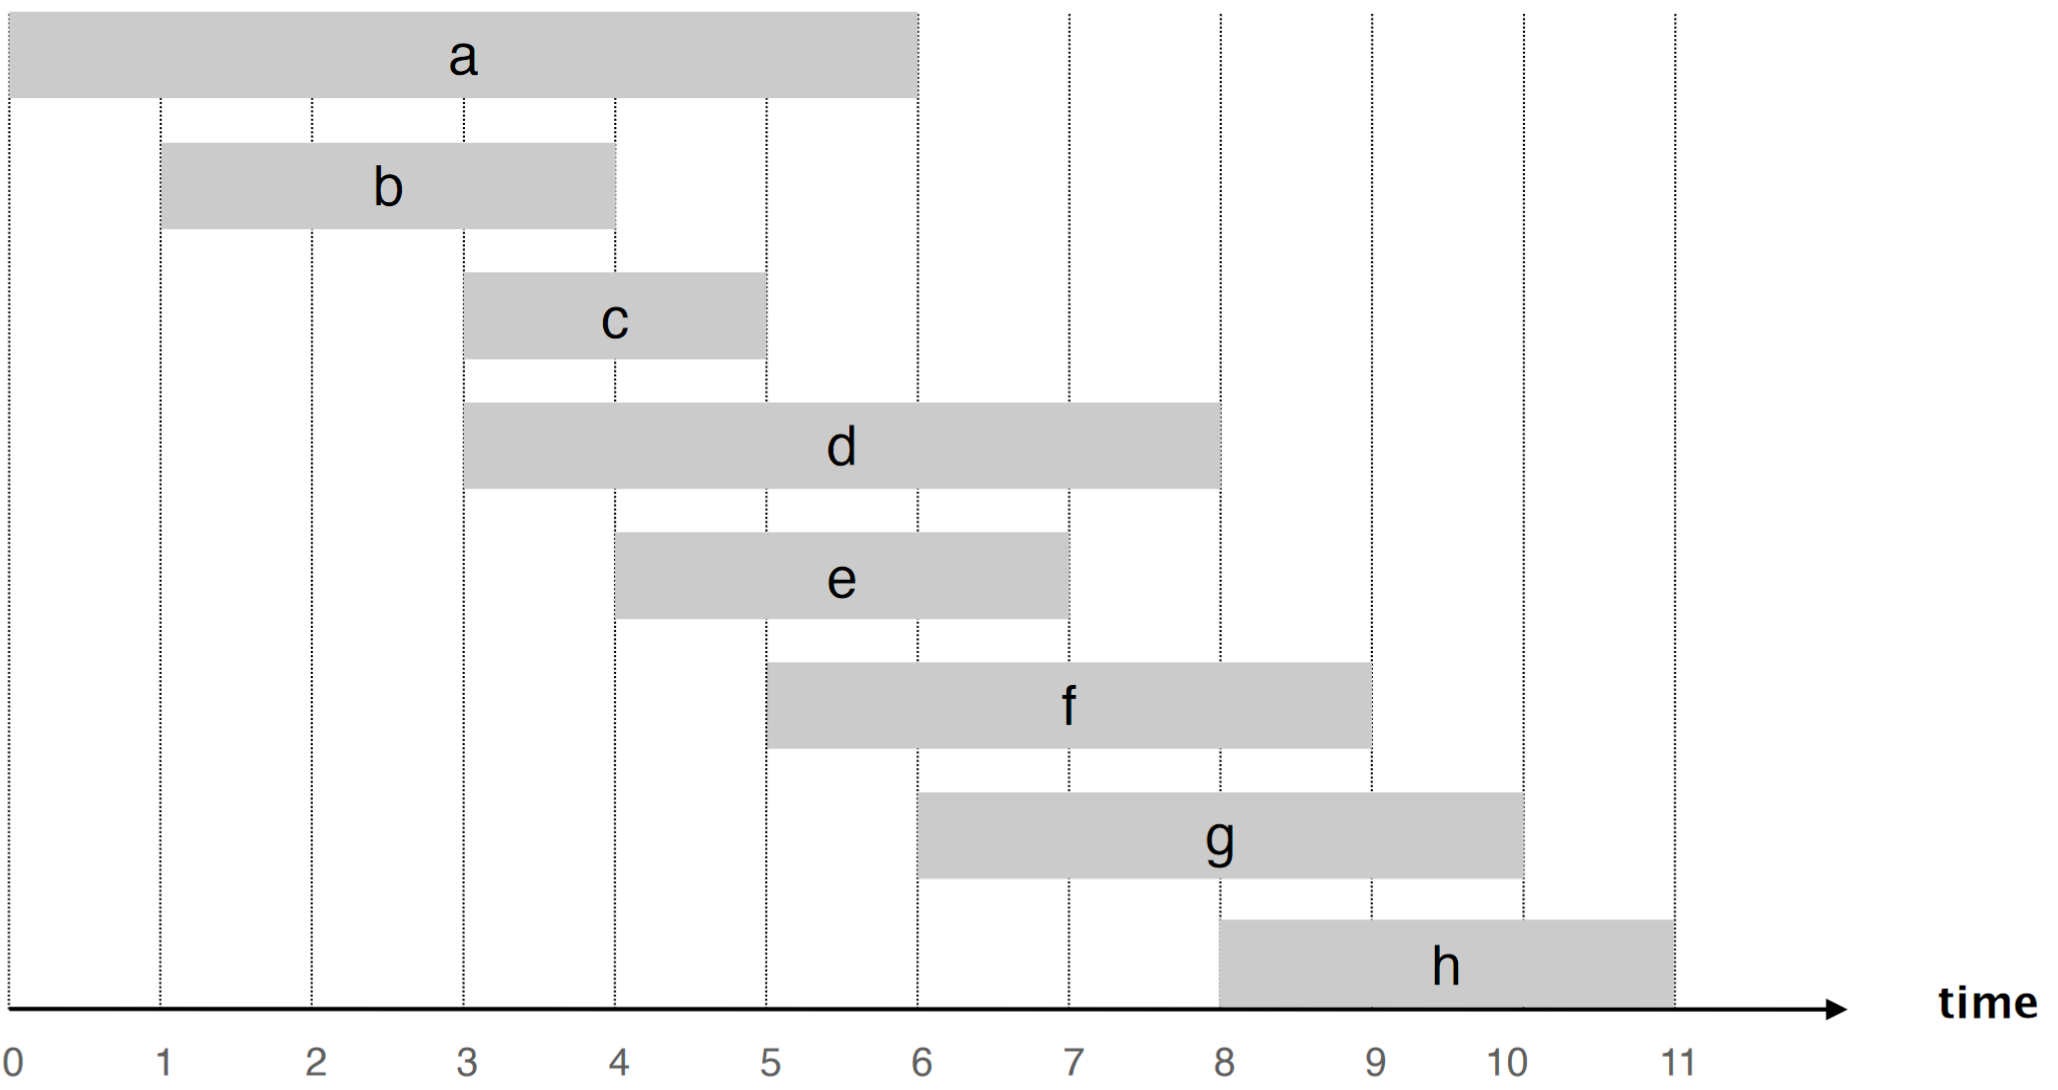
\includegraphics[height=3in]{./Sections/sched/interval/interval.png}
    \end{center}
     \caption{Given jobs $a$ through $h$ we find the largest subset of mutually compatible jobs $\{b,e,h\}$.}\label{fig:interval}
\end{figure}

\newpage

\begin{Def}[Greedy Algorithm]
    A \textbf{greedy algorithm} is an algorithm that makes the best choice at each step. I.e.,
    it cares not about the future or big picture, only the immediate benefit, for fast computations.
\end{Def}

\begin{Note}
    \textbf{Note:} This definition becomes \textit{loose}, as we encounter problems with backtracking or multiple states. As in each state
    it makes the best choice with the information available.
\end{Note}

\textbf{Possible Approaches:} Let $s_j$ and $f_j$ be the start and finish times of job $j$.
\begin{itemize}
    \item \textbf{[Earliest Start Time]:} Consider jobs in ascending order of $s_j$.
    \item \textbf{[Earliest Finish Time]:} Consider jobs in ascending order of $f_j$.
    \item \textbf{[Shortest Interval]:} Consider jobs in ascending order of $f_j - s_j$.
    \item \textbf{[Fewest Conflicts]:} For each $j$, count the number of conflicting jobs $c_j$. \par
    \hspace{9.3em} Schedule in ascending order of $c_j$.
\end{itemize}
\noindent
We choose the \textbf{Earliest Finish Time} approach:
\begin{Proof}[Greedy Algorithm Earliest Finish Time Correctness]
    Let $i_1, i_2, \dots, i_k$ denote the set of jobs selected by the greedy algorithm.
    
    Let $j_1, j_2, \dots, j_m$ denote the set of jobs in an optimal solution, with
    \[
    i_1 = j_1, i_2 = j_2, \dots, i_r = j_r \text{ for the largest possible value of } r.
    \]
    \noindent
    We can swap $j_{r+1}$ for $i_{r+1}$ in the optimal schedule, and it will still remain compatible. We repeat swaps until $r = k$.
    It’s not possible that $m > k$ because $j_{k+1}$ is compatible with $i_k$.
    \end{Proof}
   \begin{figure}[h]
    \begin{center}
      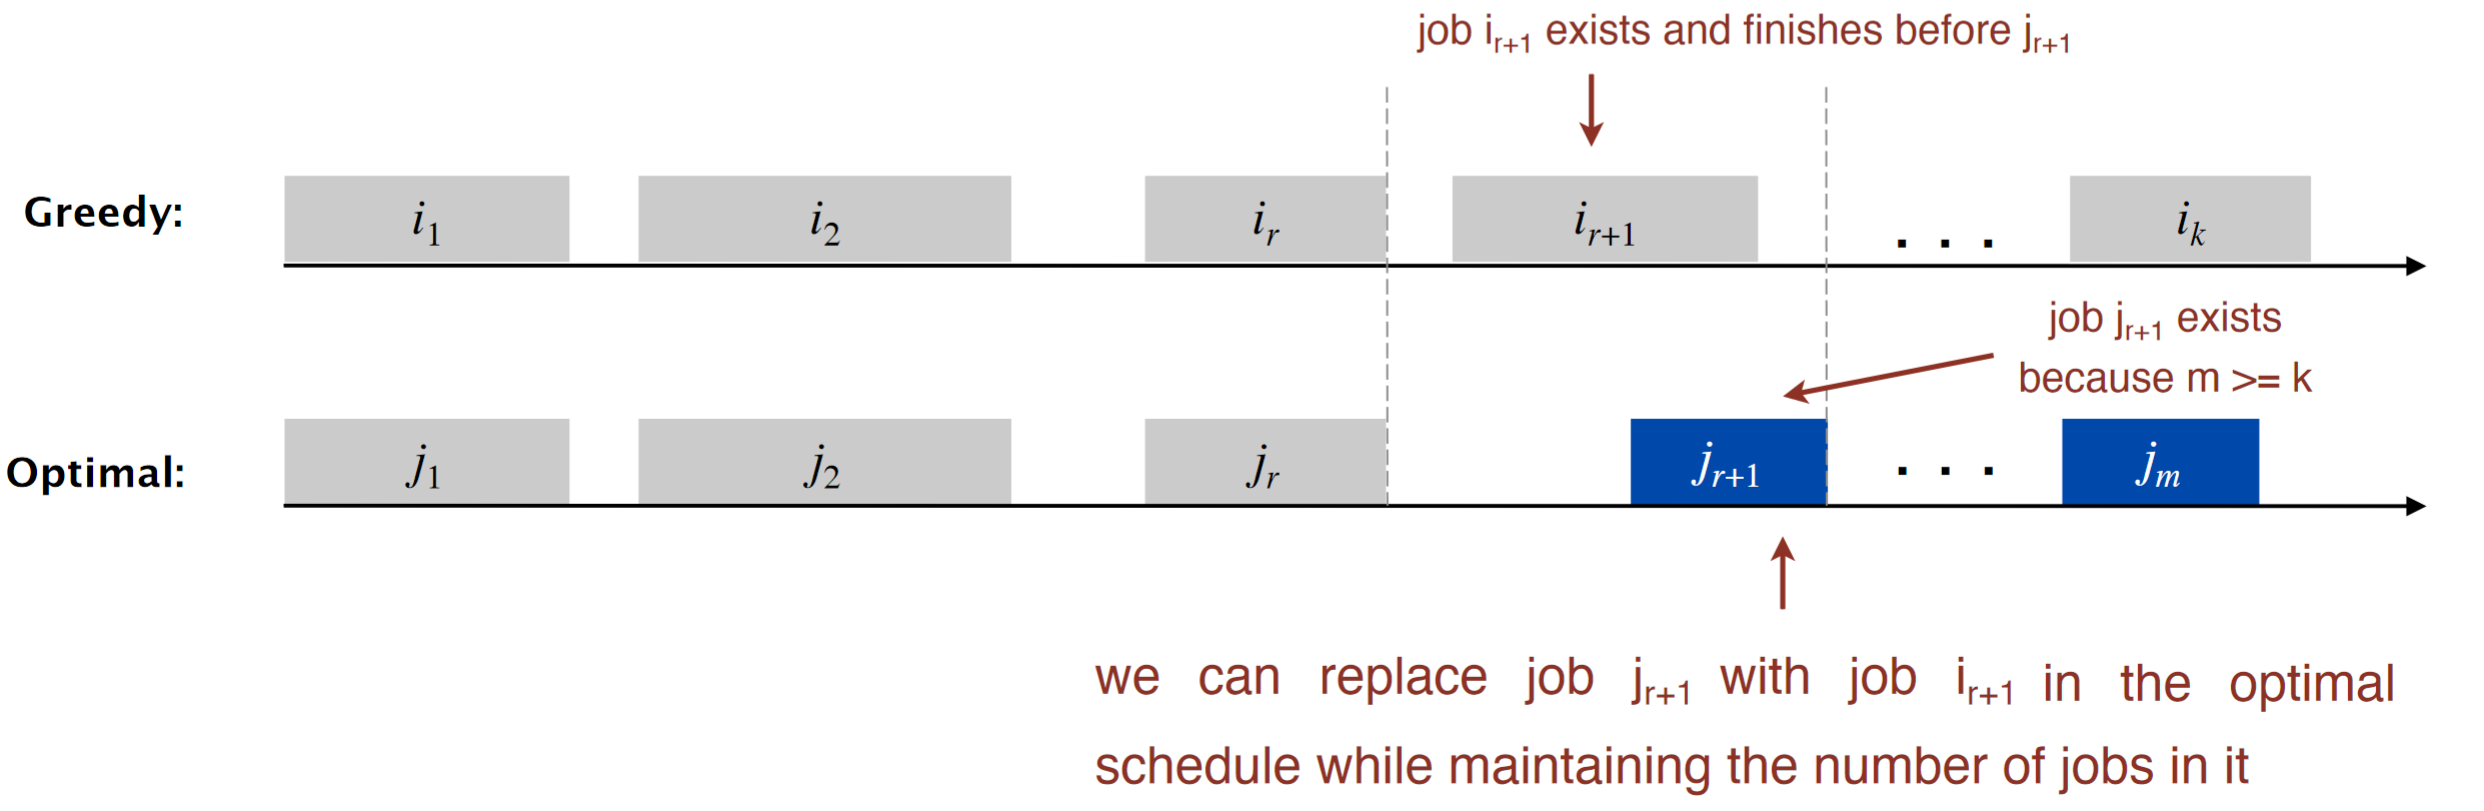
\includegraphics[height=1.7in]{./Sections/sched/interval/interval_proof.png}
    \end{center}
     \caption{Shows that at the first divergence, $i_{r+1}$ and .}\label{fig:interval_proof}
\end{figure}

\newpage 

\noindent
\begin{theo}[Interval Scheduling \& Earliest Finish Time]
    Given a set of jobs $j$ with start and finish times $s_j$ and $f_j$, we can obtain an optimal like solution by scheduling in ascending order of $f_j$,
    choosing the next compatible job.
\end{theo}
\begin{figure}[h]
    \begin{center}
      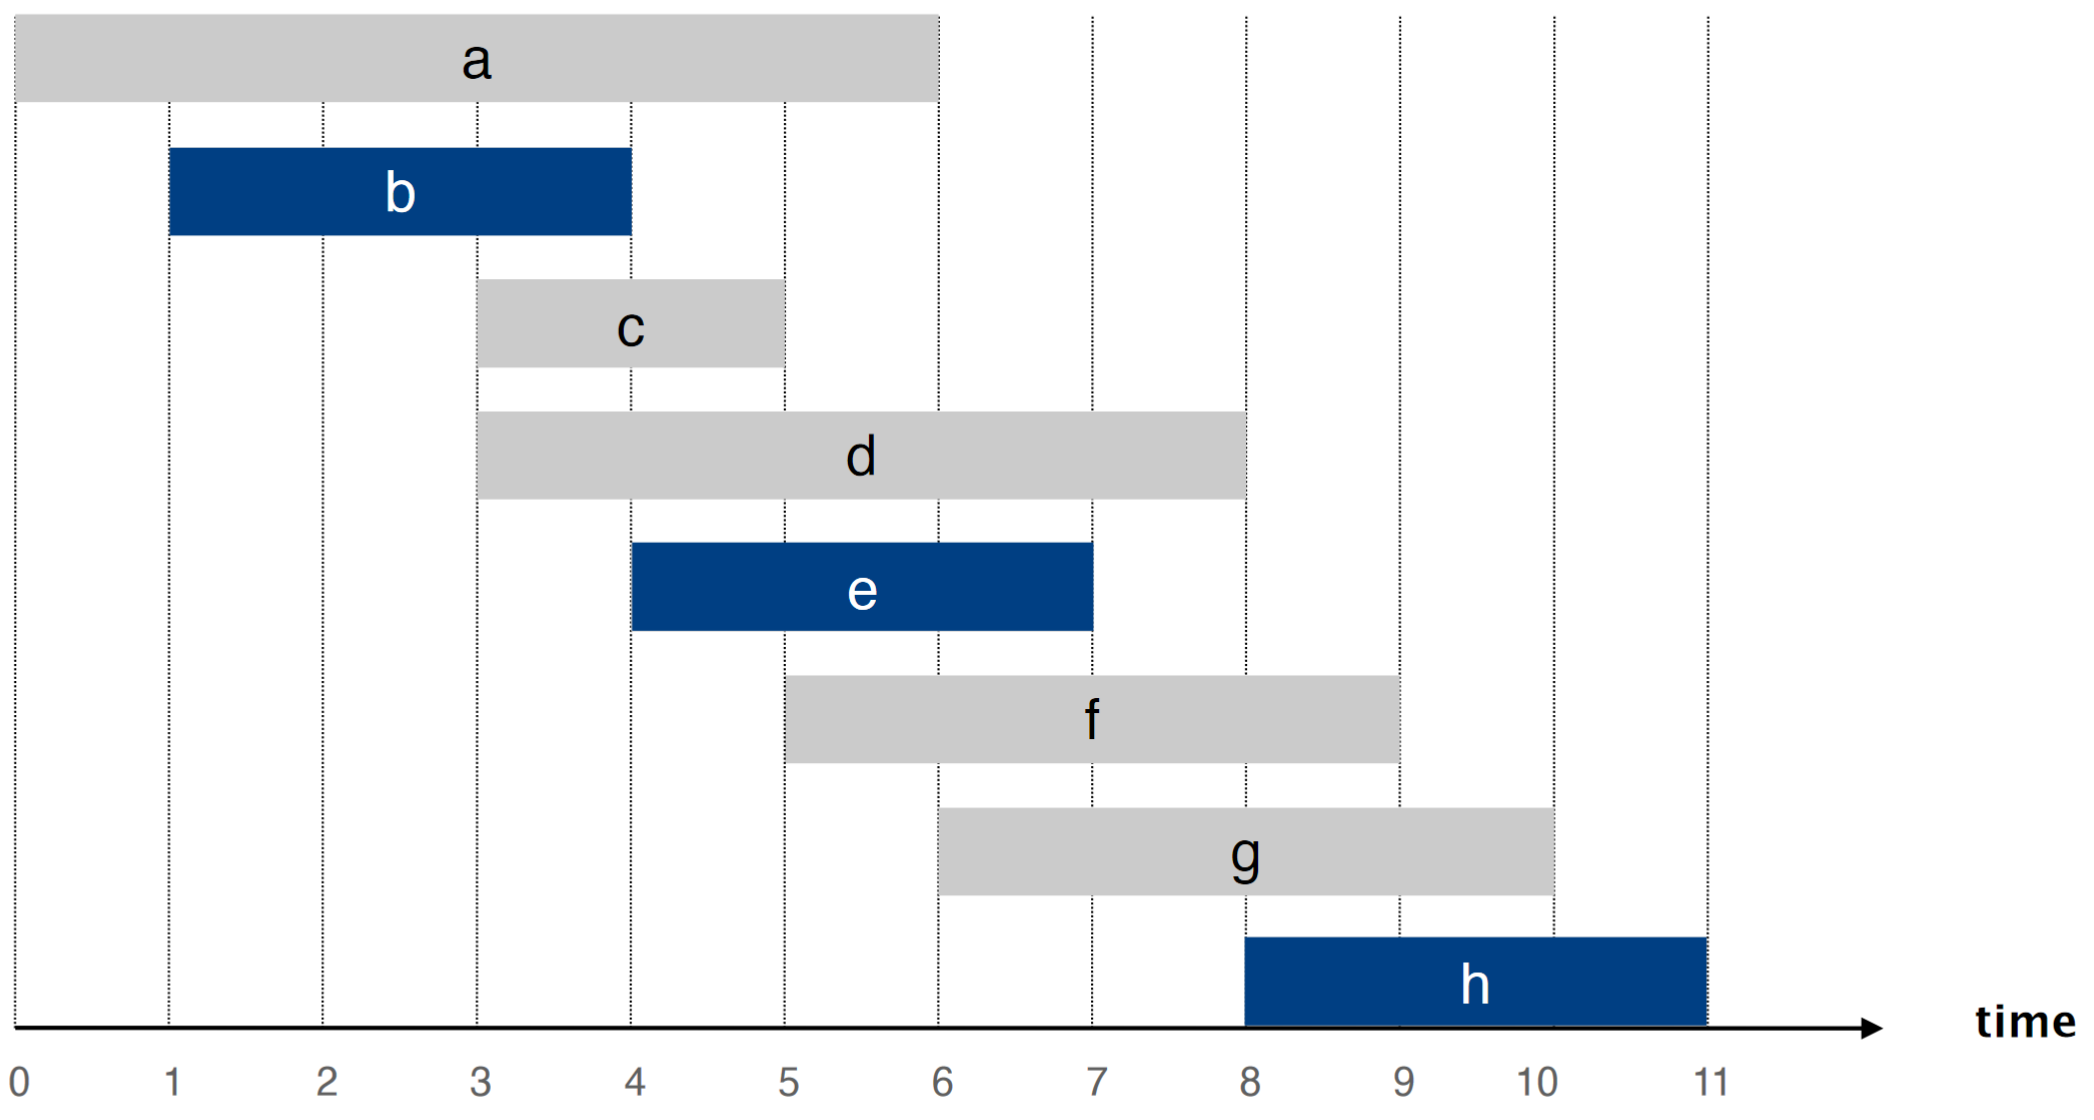
\includegraphics[height=2.5in]{./Sections/sched/interval/interval_sol.png}
    \end{center}
     \caption{Solution to Figure (\ref{fig:interval}) using early finish time first, yielding $\{b,e,h\}$.}\label{fig:interval_sol}
\end{figure}
\section{Interval Partitioning}
Interval partitioning generalizes our interval scheduling to multiple resources, allowing them to run in parallel.\\

\begin{Def}[Interval Partitioning]
    Given a schedule of jobs $j$ with start and finish times $s_j$ and $f_j$. We \textbf{partition} jobs into a minimal amount of $k$ resources such that no two jobs on the same resource overlap.
\end{Def}
\textbf{Scenerio: \textit{Class Scheduling}}\\
\noindent
Say we have $n$ classes and $k$ classrooms. What are the minimum number of classrooms needed to schedule all classes?\\

